\documentclass[tikz]{standalone}
\usepackage{amsmath}
\usepackage{xcolor}
\definecolor{bg}{HTML}{171D2B}
\definecolor{acc}{HTML}{F7B538}
\definecolor{dot}{HTML}{94A3B8}
\begin{document}
\pagecolor{bg}
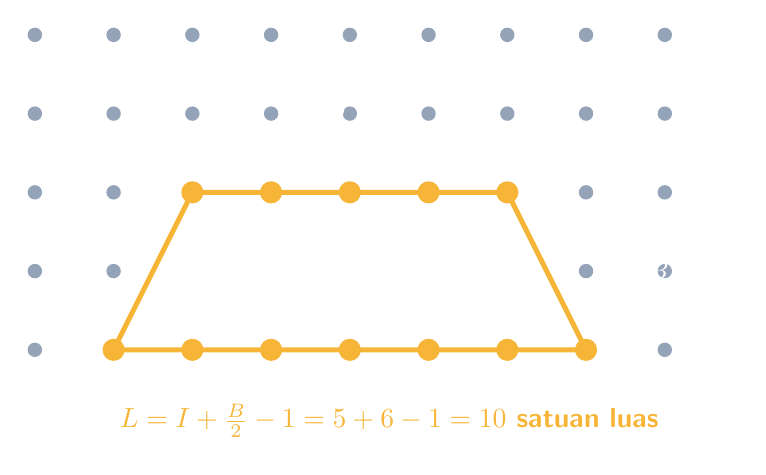
\begin{tikzpicture}[x=1cm,y=1cm, line width=1.4pt]
  \foreach \x in {0,...,8}
    \foreach \y in {0,...,4}
      \fill[dot] (\x,\y) circle (2.6pt);
  \draw[acc, line width=1.8pt, rounded corners=1pt]
    (1,0) -- (7,0) -- (6,2) -- (2,2) -- cycle;
  \foreach \p in {(1,0),(2,0),(3,0),(4,0),(5,0),(6,0),(7,0),(2,2),(3,2),(4,2),(5,2),(6,2)}
    \fill[acc] \p circle (4pt);
  \foreach \p in {(2,1),(3,1),(4,1),(5,1),(6,1)}
    \fill[white] \p circle (4pt);
  \node[white, font=\sffamily\small] at (8.3,1) {$B=12$};
  \node[white, font=\sffamily\small] at (4.2,3.0) {$I=5$};
  \node[acc, font=\sffamily\bfseries] at (4.5,-0.9)
    {$L = I + \tfrac{B}{2} - 1 = 5 + 6 - 1 = 10$ satuan luas};
\end{tikzpicture}
\end{document}
